%# -*- coding: utf-8-unix -*-
%%==================================================
%% chapter_3.tex for SJTU Master Thesis
%%==================================================

\chapter{基于数学统计策略来优化链路延时误差}
\label{chap:statistical_delay}
依据IEEE1588协议可以知道,当从时钟收到Sync报文后,会立即开始本地计算以获取主从偏差offset值。在该计算过程中,我们为了获取链路延时delay,需要假设报文往返路径对称,并利用均值的方法来获取该delay值。然而,在实际的工业现场中,由于多方面因素,如延时固有抖动、报文的排队和堵塞等,都会导致往返的链路并不对称。因此,如果想要达到亚微秒级别的同步精度,那么目前真实链路的不对称性已经成为了至关重要的瓶颈。如果无法良好的真实链路延时估计,那么无论软硬件层面进行怎样的优化,都无法真正达到亚微秒级别的同步精度,因此,本人也将在当前章节对链路延时进行深入探究。

在本章中,本人将首先简要介绍链路延时的实际影响因素,然后,针对链路延时建立完整细致的数学模型,并对该数学模型进行分析和深入研究。随后,本人将从数学统计的角度出发,将链路延时作为一系列样本值,并在从时钟处依靠时延历史样本值,估计出真正的链路延时,最终对此提出一套较为完整的解决策略。

\section{链路延时不对称性分析及其对同步精度的影响}
在第\ref{chap:1588_theory}章中,本人已经对时钟同步算法进行过详细的介绍。下面对造成链路延时不对称的几个主要因素进行详细介绍和分析。
\subsection{报文排队与堵塞}
在同步过程中,一般而言,主从时钟之间的报文传递会穿越一些中间设备如交换机或路由器等设备,而这些设备存在的主要作用是转发同步报文。可想而知,一个报文从进入该设备直到离开所消耗的时间必定是链路传输延时的一部分,相比简单的直线线路传输,该中转过程对链路延时变化有着极为重要的影响。下面将报文驻留于中间设备的总驻留时间分解成排队和堵塞两部分介绍。
\subsubsection{报文排队}
当报文进入一个如交换机的中间设备时,它会首先进入报文队列缓冲区,所有外界进入的报文都会首先进入该队列中,然后交换机系统会依次把报文取出处理并继续对外转发。当网络负载情况良好时,交换机会有很快的响应速度,即报文一进入队列缓冲区就可以立即得到转发处理。

然而,在真实的工业网络环境中,网络负载总是在实时变化的。

一旦交换机内部负载过大,队列缓冲区堆积了较多的待转发报文时,新进入的同步报文则会保持在队列末尾进行排队等待,直到交换机把前面的所有报文都转发处理了才轮到该同步报文转发。而在这个等待过程中所消耗的时间完全取决于网络负载情况和交换机内部队列的密度,这种时间对于从时钟而言是完全无法预知的。所以,很有可能前后两次的往返报文在穿越中间某个交换设备时,所消耗的等待时间会有很大差异,而正是这种差异的存在,即报文排队时间的不可预知性和随机性,导致了链路延时的不对称性。

\subsubsection{报文堵塞}
据上一部分可知,当报文进入中间交换设备时,会先进行排队等待。那么假设现在,队列中位于该同步报文之前的所有报文都已经得到了转发处理,此时轮到了该同步报文的转发操作。然而,该转发操作并非瞬间完成的。当报文进入交换设备,会依赖于该交换设备的协议栈并得到解包和打包处理。所谓解包即交换设备根据自身协议栈把报文层层解析得到用户数据,打包即重新把用户数据封装并向协议栈底层传递。这个过程我们称之为“堵塞时间”,即交换设备空闲,但由于协议栈的存在导致报文必须驻留的解析时间。

所以,在报文得到处理到真正离开中间设备,中间必须经过一段堵塞时间。

而我们知道,堵塞过程中的解包和打包操作,均需要操作系统分配CPU来进行处理。而操作系统的调度是完全随机的,我们无法提前预知操作系统的调度策略,也无法预知该解析过程所真实需要耗费的时间。尽管这些时间非常微小,但对于想要达到亚微秒同步精度的同步系统而言,这样的时间偏差不可忽视。

\subsection{网络传输抖动}
在网络系统中,所有信息的传递过程所消耗的时间会存在固有的抖动,这时无法避免的。
传统观念认为,网络流量随机过程符合马尔可夫模型或者泊松分布。其中,马尔可夫模型表示对历史具有有限的记忆,或者说在已经知道“现在”的前提下,其“将来”并不依赖于“过去”;而泊松过程中的随机变量(单位时间呼叫达到的次数)是独立且服从自相似分布的:
\begin {align}
P(X_{k} = n) = \frac{n\lambda\Delta t e^{- \lambda\Delta t}}{n!},n\geq 0;
\end{align}
然而,Vern Paxson\supercite{13}、Water Willinger\supercite{14}、Will Leland\supercite{15}及J.Beran\supercite{16}等人通过试验测量分析认为,网络流量序列在很宽的时间尺度内存在突发现象,或者说,Internet网络流量序列符合自相似特性,即样本均值的方差比样本个数的倒数减小得更慢。在此基础上,Qiong Li和David\supercite{17}又对于NTP\footnote{Network Time Protocol}时间包全程延时作了大量研究,Michael S.Borella\supercite{18}也利用两主机之间通过传送带时间标签的UDP包测量全程延时,他们都得到了相同的结论,即认为Internet网络流量及延时具有自相似特性。而以太网是构成Internet网的主要部分,所以我们有理由认为以太网网络流量及延时也具备自相似特性。

所以说,报文在以太网中传输会带有固有抖动,这也导致往返的链路延时不一定对称。

\subsection{网络拓扑结构变化}
一般的拓扑结构如图\ref{fig:1588_sync_topology}所示:

\begin{figure}[!hbp]
  \centering
  \begin{minipage}[b]{0.6\textwidth}
    \captionstyle{\centering}
    \centering
    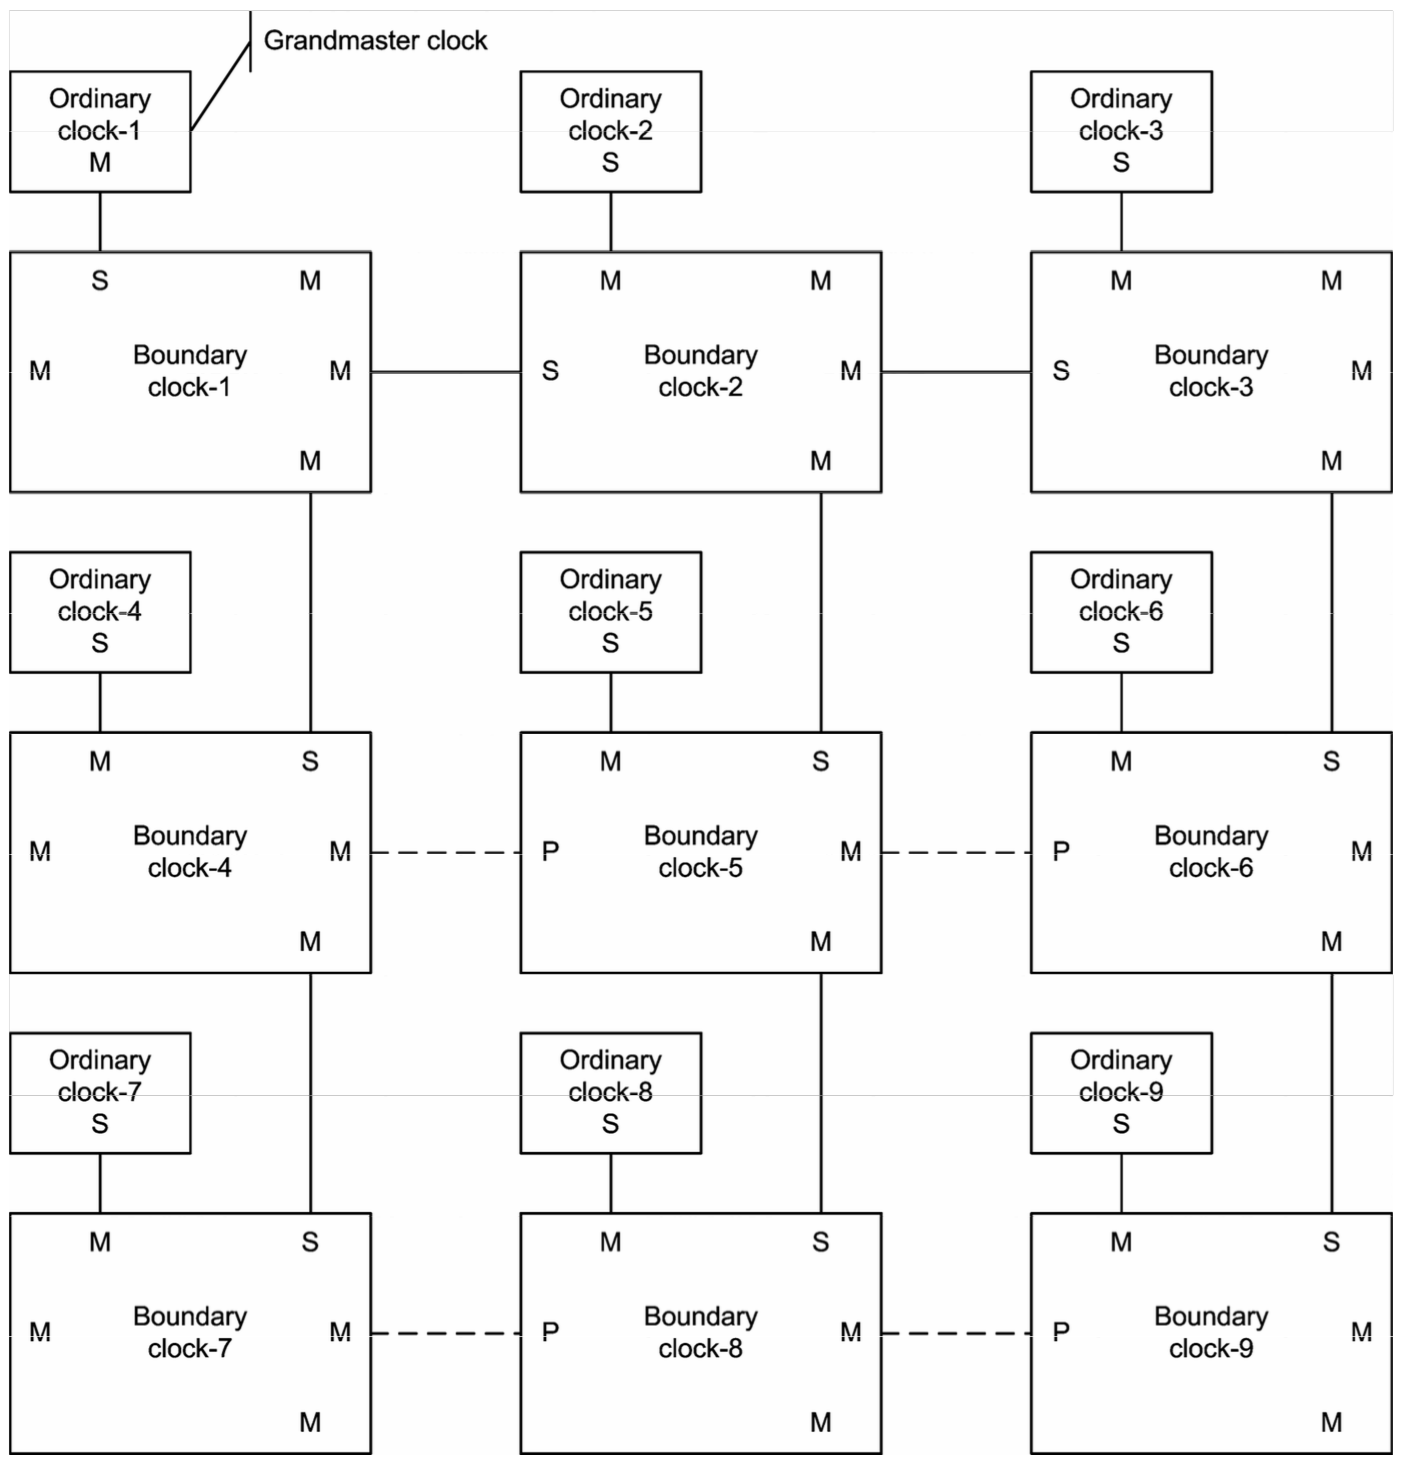
\includegraphics[width=10cm]{1588_sync_topology}
    \bicaption[fig:1588_sync_topology]{分布式同步系统结构图}{分布式同步系统结构图}{Fig}{The Structure of distributed sync system}
  \end{minipage}     
\end{figure}

假如同步系统中由于环路结构的快速重配置等原因导致链路的拓扑结构发生改变,那么肯定会导致报文传输的往返延时完全不同,而这也导致计算出来的延时值与实际值有很大偏差。然而,在现有的IEEE1588协议中,并没有很好的去探测链路结构的变化并针对性做出处理。而这一点,也正是本人下文中所针对的一个重点研究内容,并在下文中提出了相关的基于历史延时样本的应对措施。

\subsection{delay与当前真实延时不匹配}
因为delay的计算依靠Delay\_Req报文周期,而offset的计算又是依靠Sync报文周期,两者一般并不一致。所以会导致在计算offset所使用的delay是过去的值,与当前真实的delay值可能并不一致。所以,这会导致多数时候计算所使用的delay值并不一定等于真实的delay值,从而出现误差。

\section{针对链路延时进行数学建模并深入探究}
上文已经对链路延时的不对称性及其原因进行了深入的剖析。下文中,本人将针对链路延时建立数学模型,将链路延时的误差拆解到各个数学因子当中,并通过分析该数学模型进一步解析链路延时的变化,并根据数学模型的特征继续深入研究相应的解决方案。
我们知道,对于一次报文的传输过程,它所受到的影响因素主要有以下几点:
\begin{itemize}[noitemsep,topsep=0pt,parsep=0pt,partopsep=0pt]
	\item 报文排队堵塞延时:这种情况是随机的,由网络状况决定,无法预知。当网络良好时,该延时时间非常短,假设为T0;但当网络负载加剧,则延时会突然剧烈增大为T1;一旦网络恢复,则延时也跟随恢复到T0。所以,这种情况导致的延时增大往往是暂时性的。当然,在极端情况下,假设网络持续很长时间的严重负载,则延时保持T1,此时可以把这种现象视作拓扑结构变化导致的持久性变化。具体见下文,此处不过多赘述。
	\item 延时固有抖动:该抖动会导致延时发生固有的小幅波动。
	\item 拓扑结构变化或网络重配置:当拓扑结构发生变化,那么链路传输延时则与之前的延时会发生明显变化,而且之后链路延时便会保持新的延时值。所以在这里可以认为发生了持久性变化,即新延时不再与旧有延时有任何关系。
\end{itemize}

通过对链路传输延时的分析,我们可以用下列数学模型来进行描述链路传输延时:
\begin {align}
T_{all}(i) = T_{pure}(i) + T_{queue}(i) + T_{jitter}(i)
\end{align}
其中,i表示同步过程中的第i次报文传输\footnote{由于下文中会把所有延时值作为样本存储,故作此标记,i=1,2,3...},$T_{all}$代表单次链路传输总延时,$T_{pure}$代表在不考虑任何排队和抖动的情况下,在固定传输路径上的延时,$T_{queue}$代表在该次链路传输过程中,发生的排队等导致的总延时,$T_{jitter}$表示该次传输中存在的抖动延时。为保持简洁,用下面公式代替:
\begin {align}
T(i) = T_{p}(i) + T_{q}(i) + T_{j}(i)
\end{align}

下面,本人将对各个变量的特征结合上文研究做出分析。
\subsection{固定拓扑结构下的纯粹链路延时}
对于$T_{p}$,我们用来表示在固定的拓扑结构下,不考虑排队和抖动等外界干扰的纯粹链路延时。容易知道,只要链路保持不变,那么$T_{p}$就不会发生改变,也就是说,我们假设网络配置情况等保持一定的概率为$P_{path\_stable}$,那么$T_{p}$就为常量,即
\begin {align}
T_{p}(i+1) = T_{p}(i) \qquad probability: P_{path\_stable}
\end{align}
\begin {align}
T_{p}(i+1) \neq T_{p}(i) \qquad probability: (1-P_{path\_stable})
\end{align}
正常来说,网络重配置的概率非常小,也就是说$P_{path\_stable}$值非常小。但是,如果一旦发生了网络重配置,那么未来的延时与过去的延时将很有可能出现很大变化。

基于上述特性,在此本人将拓扑结构变化延时定义为“持久性”时延变化。

\subsection{报文传输排队堵塞延时}
对于$T_{q}(i)$,我们用来表示报文在传输过程中经过中间转换设备时的驻留时间。正常情况下,即当网络中流量负载良好时,$T_{q}(i)$会保持一个微小的驻留值,接近为零。但是,一旦网络负载突然加剧,那么$T_{q}(i)$会瞬间增大,而且网络负载越大,则$T_{q}(i)$会有越明显的突变。这直接导致的后果的前后几次测量的delay值有明显变化,从而影响到从时钟的精度。
所以,我们假设网络流量繁忙的概率为$P_{net\_busy}$,那么可以用如下公式来描述排队延时:
\begin {align}
T_{p}(i) = S(i) \cdot W(i) 
\end{align}
\begin {align}
S(i) = 1 \qquad probability: P_{net\_busy}
\end{align}
其中,$S(i)$是一个开关量,等于1的概率为$P_{net\_busy}$,或者说,当网络繁忙时,$S(i)$便为1;反之,当网络空闲时,$S(i)$便为0,即排队延时$T_{q}(i)$也为0。$W(i)$则表示真实的排队延时。不过一般而言,网络繁忙持续时间较短,所以在多数时间$T_{q}(i)$取值接近零,偶尔会发生阶跃性突变。

基于上述特性,在此本人将报文排队堵塞延时定义为“暂时性”延时突变。

\subsection{链路传输延时固有抖动}
对于$T_{j}(i)$,我们用来表示传输延时的固有抖动成分。该抖动主要基于$T_{p}$,度量真实链路传输时间对平均时间的偏差值。从宽时间序列角度来看,对于随机变量$T_{j}(i)$的期望值有如下公式:
\begin {align}
E(T_{j}(i)) = 0
\end {align}
这里,我们假设$T_{j}(i)$的方差值为$\sigma ^{2}$。$T_{j}(i)$都是独立同分布。

\subsection{链路传输延时模型分析及具体时延估计策略的提出}
上文中已经从数学模型角度,建立了多个方程来描述链路传输延时T。由于本文的根本出发点是利用“历史延时数据”作为样本来共同估计当前真实延时,即从时钟端会通过收集并保存历史时延样本,然后利用这些历史时延样本数据,采用结合“最小二乘法”、“动态阈值算法”和“滑动固定时间窗实时监控”三种算法来共同消除上述因素对延时造成的误差。

下面从“历史延时数据样本”角度切入,来对上文中所建立传输延时数学模型进行分析并提出相应的解决算法:
\begin{itemize}[noitemsep,topsep=0pt,parsep=0pt,partopsep=0pt]
	\item 链路传输固有延时$T_{j}(i)$:由于该固有延时是以太网流量中存在的随机因素,且我们可以认为$T_{j}(i)$是小幅波动的干扰噪声。这种干扰噪声会导致最终的传输延时处于小幅随机波动中。一般而言,针对此类随机变量最好的处理方法就是依靠历史样本进行滤波,因此,本人在下文中将提出“基于最小二乘法的滤波算法”,通过对历史延时样本进行线性回归,得到一条直线并以此来估计当前时延,从而滤除此类随机干扰噪声。
	\item 排队堵塞延时$T_{q}(i)$:若实际运行中突发网络负载加剧,则$T_{q}(i)$会由零突变增大,且取决于网络负载压力。不过,网络负载处于不断变化中,而且多数时候是网络畅通的。由于$T_{q}(i)$在阶跃增大后,会随着网络负载减小而恢复到旧有延时,因此,本人将这种延时变化定义为“暂时性”变化。也就是说,即使发生了网络负载加剧,旧有延时样本仍然有效,只是由于网络负载的出现导致传输延时出现了小幅阶跃信号。因此,本人在下文中提出了“基于动态阈值法的延时滤波”算法,用来消除历史延时样本中突变数据对时延估计结果的影响。
	\item 纯粹链路延时$T_{p}(i)$:在实际运行中,当网络重配置导致拓扑结构变化时,会使的$T_{p}$与之前的延时不一致,而且一般来讲不会恢复到之前的延时。这也就是说,拓扑结构变化直接导致了链路传输延时的“持久性”变化。由于本人采用的数学统计方法中需要依赖旧有延时来估计当前真实延时,所以,“持久性”变化的发生会导致旧有延时样本彻底失效。但如果在实际运行中,系统不能及时检测出“持久性”变化的发生,那么依旧采用已失效的旧有延时来进行同步计算,一定会导致误差大大增大。因此,本人在下文中提出了“滑动固定时间窗实时监控”算法,用来实时监控“持久性”变化,以实现尽快检测并迅速使旧有样本失效。
\end{itemize}

\section{基于最小二乘算法来处理时延固有抖动}
根据上文我们知道,固有抖动$T_{j}(i)$属于随机变量,而且我们可以认为在宽时间序列上,固有抖动的期望值$E(T_{j}(i))$为零。所以,针对这种特性的随机干扰噪声,采取任何一种统计方法都能够得到比较好的去噪效果。本人在此处选用了最小二乘算法,通过对多个历史延本数据进行线性回归,可以得到一条良好的直线,而我们可以利用这条直线来对当前延时进行估计。

之所以采用最小二乘算法,还有一个重要的原因是我们可以得到某时间段内时延回归直线的斜率,在下文的“滑动固定时间窗实时监控”算法中,我们将利用该直线斜率的变化来进行对“持久性”时延变化的实时监控。

\subsection{最小二乘法介绍}
根据维基百科的定义\footnote{\url{https://zh.wikipedia.org/wiki/\%E6\%9C\%80\%E5\%B0\%8F\%E4\%BA\%8C\%E4\%B9\%98\%E6\%B3\%95}},最小二乘法(又称最小平方法)是一种数学优化技术,它通过最小化误差的平方和寻找数据的最佳函数匹配。利用最小二乘法可以简便地求得未知的数据,并使得这些求得的数据与实际数据之间误差的平方和为最小。

\begin{figure}[!hbp]
  \centering
  \begin{minipage}[b]{0.6\textwidth}
    \captionstyle{\centering}
    \centering
    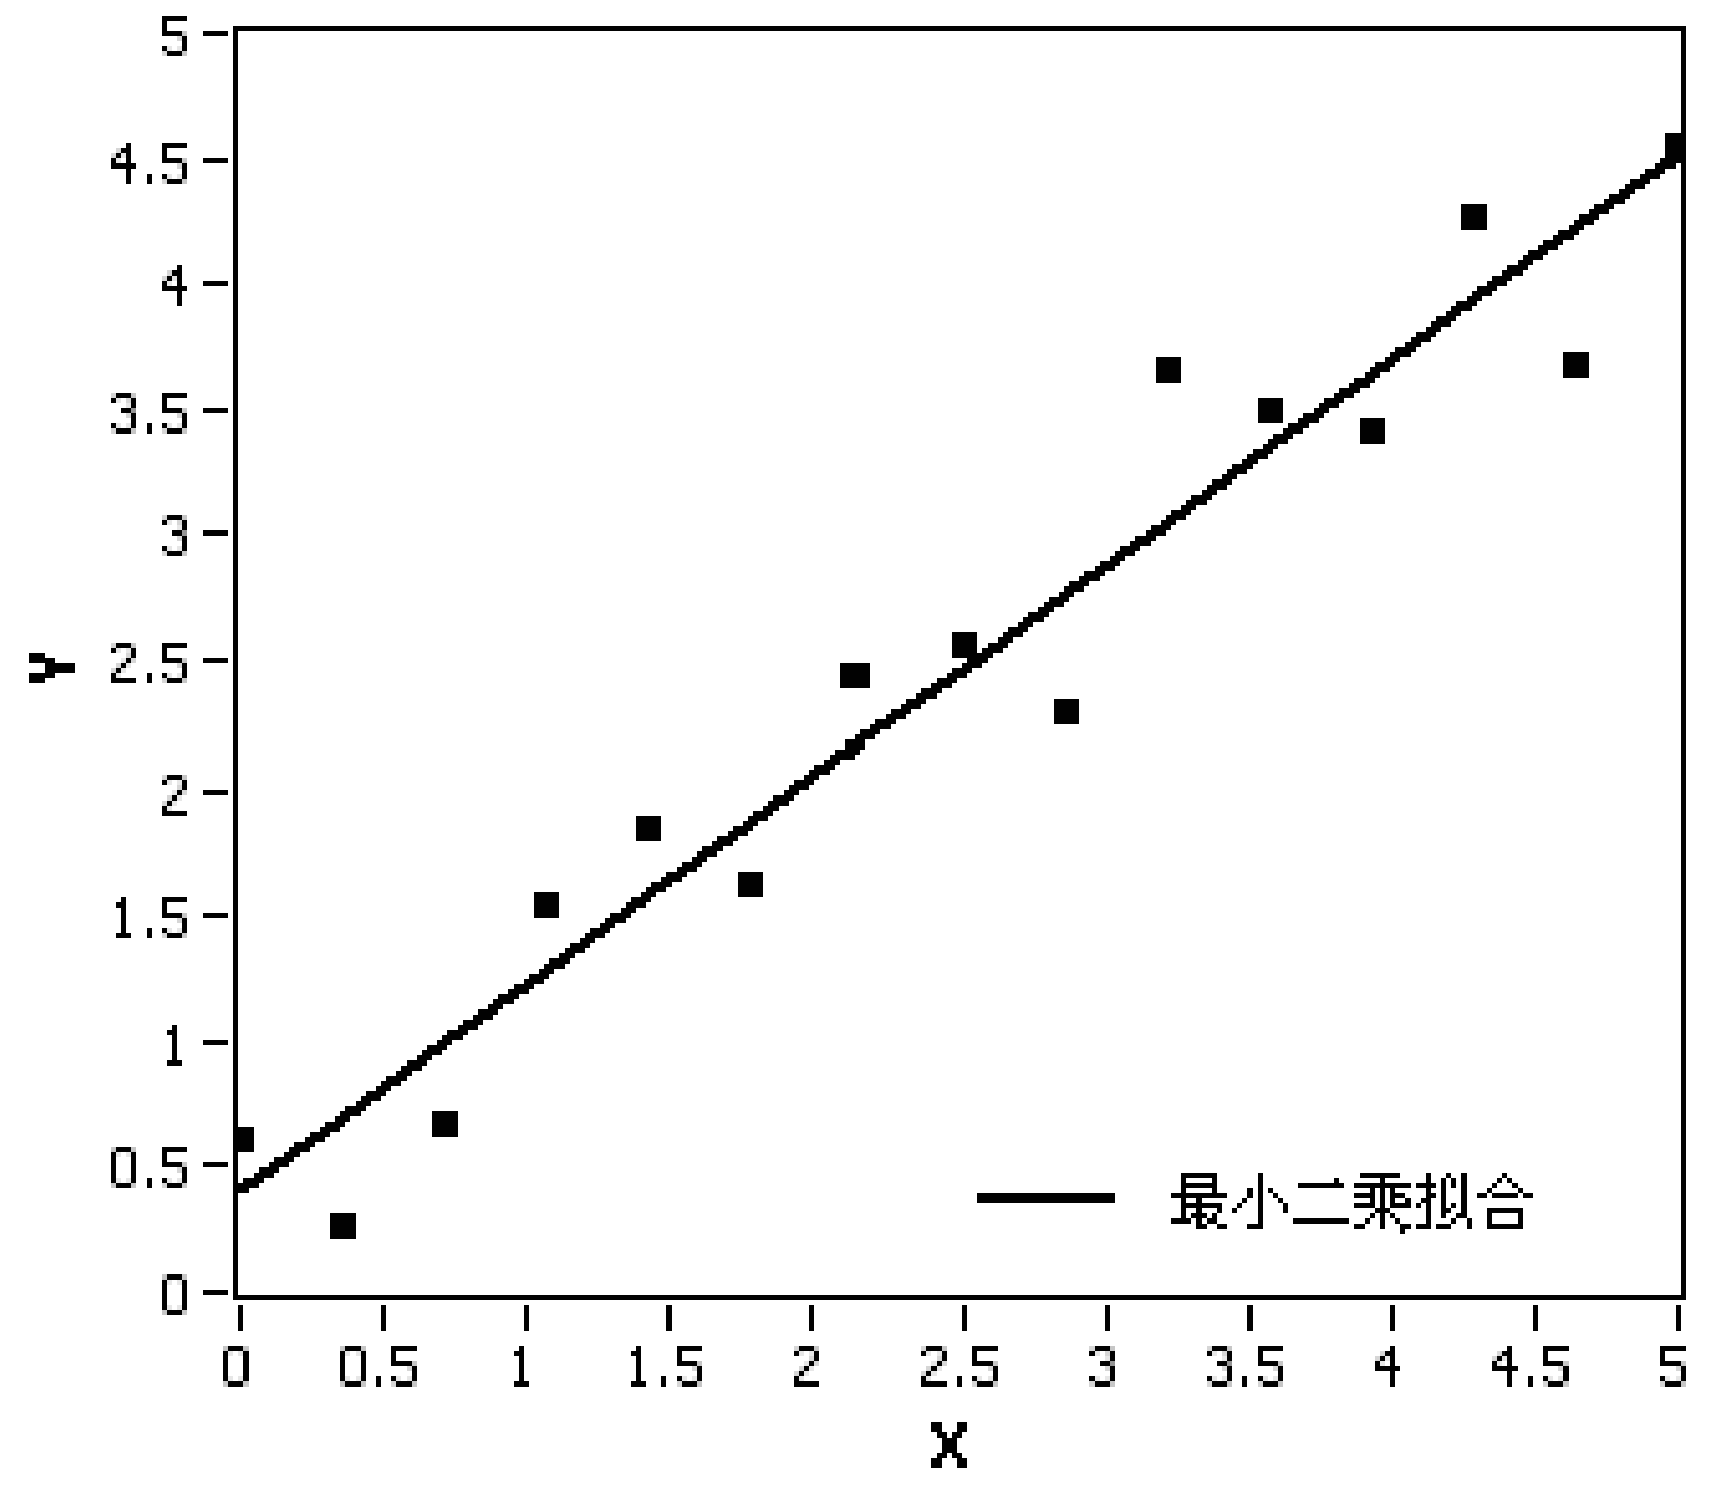
\includegraphics[width=10cm]{least_square_method}
    \bicaption[fig:least_square_method]{最小二乘法线性回归示意图}{最小二乘法线性回归示意图}{Fig}{The Least Square Method}
  \end{minipage}     
\end{figure}

\subsection{最小二乘算法实现}
在从时钟处,我们会不断收集离散的时延样本数据($t_{i}$, $D_{i}$)(i=1, 2, 3 $\cdots$),其中,$D_{i}$表示在从时钟$t_{i}$时刻获得的时延值。
为了进行最小二乘线性回归,我们取离当前最近的m个样本值来进行处理,并取基1,t,进行线性回归拟合
\begin {align}
f(t) = a_{0} + a_{1}t
\end{align}
使得方差值
\begin{align}
E(a_{0}, a_{1}) = \sum_{i=0}^{m}(f(t_{i}) - D_{i})^{2}
	= \sum_{i=0}^{m}(a_{0} + a_{1}t_{i} - D_{i})^{2}
\end{align}
能够达到极小值,因此,$a_{0}$ 和 $a_{1}$需要满足
\begin{align}
	\frac{\partial E}{\partial a_{k}} = 2 \sum_{i=0}^{m}t_{i}^{k}(a_{0} + a_{1}t_{i} - D_{i}) = 0
	\qquad(k = 0, 1)
\end{align}
上面的式子可以简化为如下形式:
\begin{align}
	a_{0}\sum_{i=0}^{m}t_{i}^{k} + a_{1}\sum_{i=0}^{m}t_{i}^{k+1} = \sum_{i=0}^{m}t_{i}^{k}D_{i}
	\qquad(k = 0, 1)
\end{align}
将该方程组转化为矩阵表示,可以得到如下的形式:
\begin{equation}
	\begin{bmatrix}
		m+1 & \sum_{i=0}^{m}t_{i} \\ 
		\sum_{i=0}^{m}t_{i} & \sum_{i=0}^{m}t_{i}^{2}
	\end{bmatrix}
	\begin{bmatrix}
	a_{0} \\ a_{1}
	\end{bmatrix}
	=
	\begin{bmatrix}
	 \sum_{i=0}^{m}D_{i} \\ \sum_{i=0}^{m}t_{i}D_{i}
	\end{bmatrix}
\end{equation}

将之前在从时钟所收集到的距当前最近的m个时延样本数据代入上述式子中,即利用方差最小原理,可以得到$a_{0}$ 和 $a_{1}$两个参数,因此便得到了一条拟合直线:f(t) = $a_{0}$ + $a_{1}$。此时,我们就可以用该直线来估计当前时刻的真实时延时,而且,由于固有抖动噪声的随机性,通过该方法会显著消除时延抖动所造成的影响。

\subsection{最小二乘算法优缺点分析}
针对链路延时固有抖动,我们由上文数学模型可以知道该抖动时属于随机变量,所以我们的思路是采用数学统计方法,把历史时延样本作为基础,通过对这些时延样本建立线性回归模型并得到一条拟合直线,通过该直线可以讲随机扰动噪声造成的影响大大减下。

但是,对于同步系统中发生的“暂时性”突变,例如由排队堵塞等导致的暂时性的时延突变,若简单最小二乘法,那么时延的突变会导致回归直线的斜率快速增大,即导致计算出来的主从偏差也快速变化。当这种“暂时性”突变恢复正常,回归直线也逐渐恢复正常。这样容易导致从时钟经常处于快速振荡状态,非常不利于从时钟系统的正常工作。

所以,在下面本人针对这种“暂时性”时延突变所带来危害进行限制,防止其突变造成主从偏差跟随性突变从而严重破坏从时钟鲁棒性。

\section{基于动态阈值法来处理“暂时性”时延变化}
由上文描述可以看出,单纯的最小二乘法确实可以有效的消除链路传输延时中的固有抖动部分,然而,一旦同步系统中发生由排队堵塞等导致的“暂时性”突变时,那么由最小二乘法回归得到的拟合直线也会随之有明显的突变,而这将导致相应的从时钟进行较大幅度的错误校正,而且,由于这种突变一般是暂时性的,所以,等网络负载恢复正常,拟合直线也渐渐恢复正常。然而,如果系统中频繁发生此类“暂时性”变化,那么势必会导致从时钟快速振荡。

因此,下文中针对“暂时性”时延变化作出深入研究,并且提出“动态阈值法”来应对此类“暂时性”变化的发生。

\subsection{“暂时性”时延变化特征研究}
对于排队堵塞等因素导致的“暂时性”时延变化$T_{q}(i)$,我们通过上文的数学模型分析可知,该时延变化因素是偶然性的,而且一般持续时间比较短,不过一旦出现,往往会导致时延出现较大的波动。我们可以将此类误差定义为“暂时性阶跃噪声”,一方面表示其持续时间较短,另一方面表示排队现象一旦发生,很有可能导致延时出现较大波动。

对从时钟而言,我们是采用上述“最小二乘法”来对历史时延进行线性回归估计,所以,如果出现了此类“暂时性阶跃噪声”,则会使的若干样本值相对旧有样本值之间,出现较大涨幅。而这种突变的涨幅会导致回归直线的斜率逐渐上升,则直接导致最终计算出来的延时值明显增大,从而导致offset值出现暂时性的大幅波动,虽然说后续随着网络负载的逐渐减轻而使的时延值及回归直线斜率逐渐恢复,但是,从从时钟稳定性角度出发,如果网络负载变化比较频繁,那么从时钟则会不断处于大幅波动之中,这对于从时钟系统稳定性极为不利。

\subsection{动态阈值法分析}
为了防止“暂时性”时延突变造成从时钟进入大幅波动甚至不稳定等现象,我们需要对时延变化进行一定的限制,或者说,我们通过历史时延的平均波动来衡量当前时延值带来的波动,如果当前时延值波动处于可接受阈值范围内则默认有效,若超过该阈值,则应该将其限制在阈值范围内。从而保持从时钟不会因为“暂时性”时延突变而出现快速大幅波动等不稳定现象。

对于阈值的选取,我们不应该将其设置为一个固定值,因为在网络环境不断变化的工业现场中我们无法提前预知排队堵塞等因素会导致的时延波动。所以,如果想要合理的判断当前时延的真实波动特性,最好的方法便是“基于历史时延波动情况”。如果当前时延波动与历史波动相比,处于一个有限范围内,那么我们可以认为当前时延带来的波动是正常的;反之,如果当前波动显著超过历史波动,那么我们应该对当前波动进行一定的限制,从而防止其对从时钟稳定性造成危害。

\subsection{动态阈值法实现}
根据上述分析可知,动态阈值的选取需要实时根据历史时延波动数据而得。所以,为了能够计算历史波动情况,本人首先创建一个固定时间窗,将每次的测量时延值保存其中;然后,通过时间窗内的历史时延值来计算时延波动阈值;最后,利用该阈值来衡量当前时延的抖动情况,并依据衡量结果来得到估计时延值。

下面给出一个含有测量时延和估计时延的固定时间窗,见表\ref{tab:dynamic_threshold}:
\begin{table}[!hpb]
  \centering
  \bicaption[tab:dynamic_threshold]{动态阈值法第k个固定时间窗}{动态阈值法第k个固定时间窗}{Table}{Mixed Time Window of Dynamic Threshold Method}
  \begin{tabular}{llllll} \toprule
  	时间 & $t_{k1}$ & $t_{k2}$ & $\cdots$ & $t_{k(m-1)}$ & $t_{km}$ \\ \midrule
    当前测量时延 & $d_{k1}$ & $d_{k2}$ & $\cdots$ & $d_{k(m-1)}$ & $d_{km}$ \\ \midrule
    动态阈值法时延估计值 & $\overline{D_{k1}}$ & $\overline{D_{k2}}$ & $\cdots$ & $\overline{D_{k(m-1)}}$ & $\overline{D_{km}}$  \\ \bottomrule
  \end{tabular}
\end{table}

算法基本思路:假设当前为时间$t_{ki}$,此时测量时延为$D_{ki}$,为了了解该时延的波动性,我们需要先计算历史时延的波动标准差,此时,假设之前的波动标准差为$\sigma_{i}$,该标准差可以直接对从$t_{k1}$时刻到$t_{k(i-1)}$时刻之间的估计时延,依据标准差公式计算而得。此处不作赘述。然后,我们可以依据该标准差$\sigma_{i}$来选取我们的动态阈值,依据下式来进行选取:
\begin{align}
T_{i} = \alpha * \sigma_{i}
\end{align}
其中,$T_{i}$表示在$t_{ki}$根据历史时延数据实时计算出来的当前动态阈值\footnote{Dynamic Threshold},我们可以认为通过设定参数$\alpha$来调节阈值的范围。

然后,我们还需要引入截止函数来判断当前波动是否超出动态阈值的范围,并根据判断结果做出相应处理方法。本人采用如下截止函数,当波动超过动态阈值时则直接取该阈值来计算当前实验估计值。
\begin{equation}
G(d_{i}) = \left\{
	\begin{array}{lll} % \begin{eqnarray}好像也可以。
		d_{i}, \qquad \left | d_{i} \right | < \alpha * \sigma_{i} \\
		\alpha * \sigma_{i}, \quad d_{i} \geq \alpha * \sigma_{i} \\
		-\alpha * \sigma_{i}, \quad d_{i} \leq -\alpha * \sigma_{i}
	\end{array}
	\alpha > 0 \right. 
\end{equation}

基于上面的动态阈值与截止函数,在$t_{ki}$时刻,我们可以利用第k个固定时间窗历史数据及当前测量延时$d_{i}$得到如下当前时延估计值:
\begin{align}
\overline{D_{ki}} = \gamma * G(d_{i}) + \overline{D_{k(i-1)}}; \qquad 1\leq i \leq m
\end{align}
其中,$\gamma$用来表示当前测量时延在当前估计时延$\overline{D_{ki}}$中所占的比重,一般可以取:
\begin{align}
\gamma \approx (0.85-0.9)
\end{align}
最后,每一轮时间窗的第一个延时估计值$\overline{D_{k1}}$是取上一轮时间窗所有时延估计值的平均值,即:
\begin{align}
\overline{D_{k1}} = \frac{1}{m} * \sum_{i=1}^{m}\overline{D_{(k-1)(i)}}
\end{align}

\subsection{动态阈值法优缺点分析}
利用上述动态阈值法,我们可以通过在固定时间窗内,通过计算历史时延值来得到一个动态阈值,然后利用该动态阈值来衡量当前测量时延的波动影响。若链路中发生较为严重的排队堵塞延时,导致时延值突然大幅增大,那么可以通过该动态阈值方法可以有效防止时延值大幅突变对从时钟造成的快速振荡甚至不稳定,从而使得从时钟有更佳优良的稳定性。

但是,此方法的前提是该时延突变必须为“暂时性”突变,也就是说这种突变只是短时间内的,随着系统继续运行该突变又会逐渐减小并恢复正常。只有在这样的前提下,我们才可以通过动态阈值限定方法,在这个突变的短时间内把时延突变对从时钟造成的影响尽量减小。

然而,如果同步系统中发生的是“持久性”突变,例如拓扑结构变化,那么就意味着真实时延值与历史时延值已经完全不同,如果此时仍然采用上述动态阈值法强制把时延限制在一个有限范围内,那么很有可能导致数据完全偏离真实时延,出现难以想象的错误。

基于此,下面继续针对同步系统中可能发生的“持久性”时延变化提出一种实时监控算法,该算法能够快速发现“持久性”突变的发生,并且立即通过使历史样本失效的方法来刷新时间窗并重新进行时延估计。

\section{提出滑动时间窗实时监控算法来处理“持久性”延时变化}
\subsection{“持久性”延时变化特征研究}
由上文可以看出,基于“最小二乘法”和“动态阈值法”可以有效的消除固定抖动噪声和“暂时性”阶跃噪声,改善了同步系统的精确性和鲁棒性。但是,如果发生由网络重配置等因素导致的拓扑结构变化时,就会导致链路传输时延的“持久性”变化,如果仅仅采用上述两种方法是无法有效应对此类变化的。

根本原因在于,一旦发生“持久性”变化,则意味着历史延时样本均已经失效,不应该继续用于后续的时延估计中。然而,上述两种方法均依赖于历史延时样本,而且这两种方法均无法探测出“持久性”变化的发生。这样带来的直接后果就是:在时延已经完全变化后,同步系统仍然继续使用错误的历史延时样本数据去估计当前真实的延时,所计算出来的估计时延值一定会与真实时延存在很大偏差,而且这样的偏差要一直持续到右足够多的新样本替代旧有时延样本后才能逐渐消除。

显然,这会严重破坏系统的同步精度和稳定性。

因此,本人提出了一种基于固定滑动时间窗的实时监控算法。下面,本人对该算法进行详细的介绍。

\subsection{滑动时间窗实时监控算法介绍}
这里所谓的“持久性”变化主要是指一旦发生了网络拓扑结构等变化,那么新的链路传输延时将与旧有延时样本完全不一致,这也就意味着,旧有累积延时样本已经不能作为我们计算新延时的基础数据了。否则,大量失效的延时样本数据会导致当前依靠最小二乘法所得到的时延估计出现非常严重的偏差。

所以,下面本人会上述最小二乘法所得到拟合直线斜率角度入手,来实时监控“持久性”变化的发生。

当从时钟收到同步报文时,会立即依靠历史数据和最小二乘法来建立一条回归直线。那么我们考虑这样一种情况,如果网络发生了重配置导致链路传输延时,那么此刻之后的新的延时数据就会与之前的样本数据有明显偏差,而此时我们仍然在使用最小二乘线性回归方法计算回归直线。那么可想而知,此刻之后的回归直线斜率会发生明显突变,假设网络重配置导致链路变得更长,那么得到的延时也就比之前更大,对应的回归直线斜率也会不断的向上提升,一直到历史实验样本全部被新的时延数据替代,那时的新的回归直线会恢复到接近水平。而在这个过程中,由于直线斜率的先增后减,导致其估计出来的时延值非常不准确,而且会导致从时钟发生一次大幅波动。

所以,理想的状态应该是,当发生拓扑结构突变,链路延时回归直线开始提升时,就能够尽快检测并发现这种现象,然后立即把历史时延数据“失效化”。从而,新的时延数据不会被历史样本影响而导致从时钟要经过长时间的波动直到新的时延完全替代旧有时延样本。于是,通过立即把历史时延数据失效的方法可以让从时钟尽快得到校正。

\subsection{滑动时间窗实时监控算法具体实现}
通过上述介绍,本人将目标着眼于回归直线斜率的变化情况,并通过对历史斜率的实时监控从而快速发现“持久性”变化的发生,并且采取使历史样本数据“立即失效”的方法来快速校正从时钟。

为了能够实时监控回归直线的“历史斜率”变化情况,下面本人会提出滑动时间窗方法来实时监控并计算斜率变化。
\begin{table}[!hpb]
  \centering
  \bicaption[tab:slide_window]{实时监控算法中在当前$t_{c}$时刻的长度为m的滑动时间窗}{在当前$t_{c}$时刻的滑动时间窗}{Table}{Slide Time Window at current time $t_{c}$ in Real-Time Monitor Method}
  \begin{tabular}{llllll} \toprule
  	时间 & $t_{c1}$ & $t_{c2}$ & $\cdots$ & $t_{c(m-1)}$ & $t_{cm}$ \\ \midrule
    当前测量时延 & $d_{c1}$ & $d_{c2}$ & $\cdots$ & $d_{(cm-1)}$ & $d_{cm}$ \\ \midrule
    当前回归直线斜率 & $\overline{K_{c1}}$ & $\overline{K_{c2}}$ & $\cdots$ & $\overline{K_{c(m-1)}}$ & $\overline{K_{cm}}$  \\ \bottomrule
  \end{tabular}
\end{table}

在表\ref{tab:slide_window}中,该时间窗最后一列数据为当前值。对应当前时刻为$t_{c}$,此时测量得到的时延值为$d_{c}$,同时可以得到当前回归直线的斜率值$\overline{K_{c}}$。我们知道,如果当前同步系统并非发生“持久性”变化,那么该回归直线的斜率值应该是接近零并处于上下小幅抖动之中;而如果同步系统发生拓扑结构等“持久性”时延变化,那么斜率值则会处于一个不断上升或者不断下降的趋势之中。其中,不断上升意味着新的拓扑结构带来了更长的链路传输延时,反之,不断下降则意味着新拓扑结构带来了更短的链路传输延时。

那么,为了监控回归直线斜率的变化,本人从该滑动时间窗内的所有斜率样本值角度出发,通过探究这些斜率样本值的波动方差来决定是否发生“持久性”变化。即利用下面的式子来计算时间窗内的斜率均值$E_{c}$和方差$D_{c}$:
\begin{align}
E_{c} = \frac{1}{m}\sum_{i=1}^{m}(\overline{K_{ci}}) \\
D_{c} = \frac{1}{m}\sum_{i=1}^{m}(\overline{K_{ci}} - E_{c}) ^ {2}
\end{align}

所以,在$t_{c}$时刻我们可以计算出时间窗内的历史斜率波动方差为$D_{c}$,根据上文分析,若该方差接近零,则表示保持小幅振荡,此时可以认为没有发生“持久性”变化;但如果斜率方差值超过一定范围,那么我们可以认为同步系统中发生了“持久性”变化,为了使系统快速适应这种变化,我们需要立即使历史样本失效。因此,我们采用下面函数来处理这种过程:
\begin{equation}
R_{c} = \left\{
	\begin{array}{ll} % \begin{eqnarray}好像也可以。
		0, \qquad D_{c} < \omega * \overline{DT} \\
		1, \quad D_{c} \geq \omega * \overline{DT} 
	\end{array}
	\right. 
\end{equation}
其中,$\omega$为可调节参数,$\overline{DT}$为指定阈值。若当前时间窗内所计算出来的波动超过了限定阈值,那么就认为发生了“持久性”变化,进行失效处理,从而保证从时钟对“持久性”变化的适应性和快速响应性。

除此之外,对于“滑动时间窗”的实现,首先我们在上文中假设该时间窗长度为m,然后我们以最新测量时刻$t_{c}$为该滑动时间窗的末尾一组数据,向前获取前(m-1)组数据加入该滑动时间窗内部。所以,每次新收到一次同步报文,便把该报文的数据加入到该滑动时间窗的最后一组,与此同时,将第一组数据从该时间窗内移除。所以整体看来,该时间窗是处于不断前行的一个过程,因此成为“滑动时间窗”。采用这样的方法可以时刻保持当前历史时延数据最新,才能够最快的监控出最真实的回归直线斜率的变动情况。

\subsection{滑动时间窗实时监控算法小结}
首先,该算法主要是用来应对同步系统链路中发生的网络重配置等导致的拓扑结构变化。由于本人是从统计角度入手,所以每次同步计算都要严重依靠历史样本数据。而如果一旦发生了上述的“持久性”变化,那么就意味着历史样本数据已经完全失去效果了,如果继续使用则会导致严重误差且长时间无法正确校正。所以,本方法通过对时延的变化情况着手,通过实时监控最小二乘法中拟合直线的斜率变化,来快速判断同步系统中是否发生了“持久性”变化,一旦发现,便立即将历史样本失效,从而能够减小这种变化对同步系统造成的危害。

\section{本章小结}
在当前工业的时钟同步系统中,对精度要求越来越高,甚至达到了亚微秒级别。而之所以IEEE1588协议在工业应用中难以达到这样的同步精度,首要的原因就是协议本身无法很好应对复杂工业环境下链路延时的无法预知的变化。该延时变化主要包含下面三种因素:
\begin{itemize}[noitemsep,topsep=0pt,parsep=0pt,partopsep=0pt]
	\item 链路传输固有延时:由于链路延时本身存在固有抖动,所以我们需要从时钟能够有效的滤除这些随机干扰噪声,但是原始的处理方案中只是简单的采用均值滤波,并不能很好的处理更复杂的情况。
	\item 排队堵塞延时:网络流量负载情况是无法预知和随机的,一旦网络负载加剧,则会导致报文延时突然变化,随着网络负载逐渐恢复,报文延时也逐渐恢复,但传统的处理方法在遇到这种情况时会使得从时钟鲁棒性很差,一直处于快速波动状态,这非常不利于从时钟系统的运行。
	\item 网络重配置导致延时更新:由于同步系统很有可能会发生网络重配置的情况,如添加新的时钟或移除,或者改变整个网络拓扑结构。而在原始的处理方案中,对于这种情况完全没有考虑,一旦发生就导致从时钟发生突然的大幅振荡,这是非常不利的。
\end{itemize}

所以,本章从链路传输延时为出发点,以数学统计方法为根本原则,对链路传输过程中可能导致时延变化的多个因素进行详细而深入的分析,并且通过对该延时建立完整的数学模型,然后通过其数学特性,依次提出了“最小二乘法”、“动态阈值法”和“滑动时间窗实时监控”等多个数学统计算法来分别处理其中的固有抖动、“暂时性”延时和“持久性”延时。这些方法都是基于历史实验样本数据,而且这几种方法互相依赖,能够完整而高效的应对复杂工业环境中同步系统链路延时的多种状况。不仅提高了从时钟的快速响应性,还大大提高了从时钟的稳定性和鲁棒性。使的同步系统能够在复杂环境下有更加优良的表现。





